% Use the xelatex engine for Unicode support
\documentclass[12pt]{article}

\usepackage[a4paper, margin=1in]{geometry}
\usepackage{graphicx}
\usepackage{amsmath}
\usepackage{booktabs}
\usepackage{caption}
\usepackage{listings}
\usepackage{xcolor}

\definecolor{codegreen}{rgb}{0,0.6,0}
\definecolor{codegray}{rgb}{0.5,0.5,0.5}
\definecolor{codepurple}{rgb}{0.58,0,0.82}
\definecolor{backcolour}{rgb}{0.95,0.95,0.92}

\lstdefinestyle{mystyle}{
    backgroundcolor=\color{backcolour},
    commentstyle=\color{codegreen},
    keywordstyle=\color{magenta},
    numberstyle=\tiny\color{codegray},
    stringstyle=\color{codepurple},
    basicstyle=\ttfamily\footnotesize,
    breakatwhitespace=false,
    breaklines=true,
    captionpos=b,
    keepspaces=true,
    numbers=left,
    numbersep=5pt,
    showspaces=false,
    showstringspaces=false,
    showtabs=false,
    tabsize=2,
    literate={--}{{-{}-}}2, % ADD THIS: To handle hyphens correctly in comments
    extendedchars=true % ADD THIS: To allow extended characters
}
\lstset{style=mystyle}

\title{Reinforcement Learning Policy Analysis in a Grid World}
\author{Wenkang Ji}

\date{\today}
\begin{document}

\maketitle

\section{Software}

The simulation and analysis were conducted using Python 3. Key scientific computing libraries utilized include:
\begin{itemize}
    \item \textbf{NumPy:} For efficient array operations and numerical calculations.
    \item \textbf{Matplotlib:} For plotting the grid world, policies, and agent trajectories.
\end{itemize}

\section{Reward Setting and Discount Rate}

The agent receives feedback from the environment in the form of rewards. The reward structure is designed to guide the agent towards the target state.

\begin{itemize}
    \item \textbf{Target Reward:} A positive reward of $R_{\text{target}} = +1.0$ is given upon reaching the target state.
    \item \textbf{Forbidden Reward:} A negative reward of $R_{\text{forbidden}} = -1.0$ is given for attempting to enter a forbidden state or moving off the grid. The agent does not move in this case.
    \item \textbf{Step Reward:} A neutral reward of $R_{\text{step}} = 0.0$ is given for any other valid move.
\end{itemize}

The \textbf{discount rate}, $\gamma$, is set to \textbf{0.9}.

\section{Policy 1: Deterministic Policy}

\subsection{Policy Description}
This policy is designed to be optimal. It is generated using a Breadth-First Search (BFS) algorithm that works backward from the target state to find the shortest path from every other valid state. For any given state, the policy deterministically selects the action that moves the agent one step along this shortest path. For terminal or unreachable states, the policy is to stay.

The policy is represented in the table below, where each cell indicates the probability of taking an action from a given state. A value of $1.00$ signifies a deterministic choice.

\begin{table}[h!]
\centering
\caption{Deterministic Policy Table}
\begin{tabular}{lccccc}
\toprule
\textbf{State (x,y)} & \textbf{(0, 1) down} & \textbf{(1, 0) right} & \textbf{(0, -1) up} & \textbf{(-1, 0) left} & \textbf{(0, 0) stay} \\
\midrule
(0, 0) & 0.00 & 1.00 & 0.00 & 0.00 & 0.00 \\
(0, 1) & 0.00 & 0.00 & 1.00 & 0.00 & 0.00 \\
(0, 2) & 0.00 & 0.00 & 1.00 & 0.00 & 0.00 \\
(1, 0) & 0.00 & 1.00 & 0.00 & 0.00 & 0.00 \\
(1, 1) & 0.00 & 0.00 & 1.00 & 0.00 & 0.00 \\
(2, 0) & 0.00 & 1.00 & 0.00 & 0.00 & 0.00 \\
(2, 2) & 0.00 & 0.00 & 0.00 & 0.00 & 1.00 \\
(3, 0) & 0.00 & 1.00 & 0.00 & 0.00 & 0.00 \\
(3, 2) & 0.00 & 0.00 & 0.00 & 1.00 & 0.00 \\
(4, 0) & 1.00 & 0.00 & 0.00 & 0.00 & 0.00 \\
(4, 1) & 1.00 & 0.00 & 0.00 & 0.00 & 0.00 \\
(4, 2) & 0.00 & 0.00 & 0.00 & 1.00 & 0.00 \\
\bottomrule
\end{tabular}
\end{table}

\subsection{Policy Plot and Trajectory}
Starting from state \textbf{(0, 2)}, the agent's trajectory over 50 steps is simulated. The policy is visualized with green arrows on the grid, and the agent's path is shown as a green line, as depicted in \textbf{Figure~\ref{fig:deterministic}}.

\begin{figure}[h!]
\centering
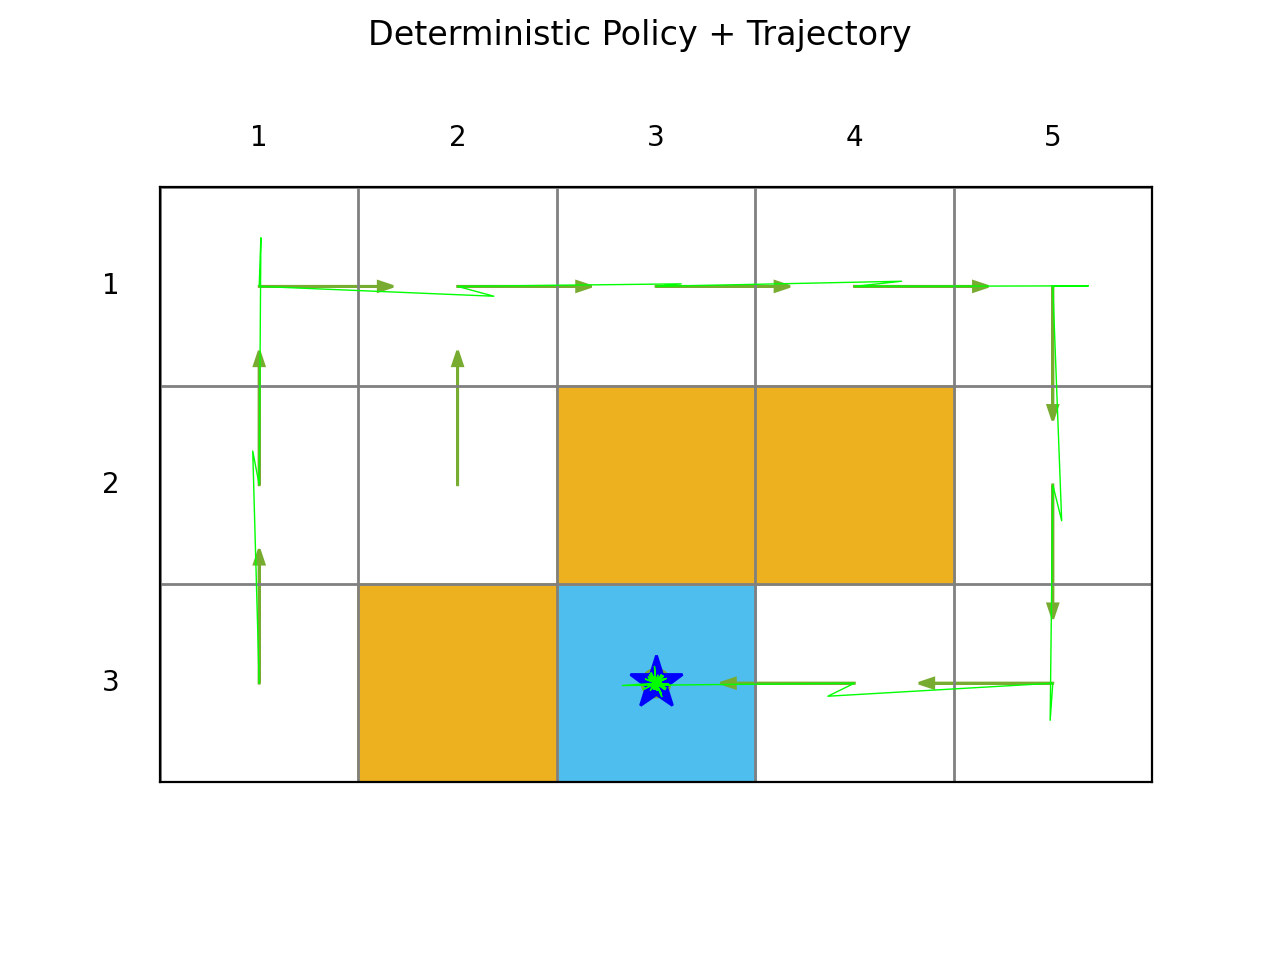
\includegraphics[width=0.7\textwidth]{deterministic_policy_trajectory.png}
\caption{Visualization of the deterministic policy (arrows) and the resulting trajectory (line) from start state (0, 2).}
\label{fig:deterministic}
\end{figure}

% Use a breakable environment for long lines
The first 10 states of the trajectory are:
\begin{verbatim}
[(0, 2), (0, 1), (0, 0), (1, 0), (2, 0),
 (3, 0), (4, 0), (4, 1), (4, 2), (3, 2)]
\end{verbatim}


\subsection{Discounted Return}
The calculated discounted return for this 50-step trajectory is:
$$ G = 3.822667137926801 $$

\newpage
\section{Policy 2: Stochastic Policy}

\subsection{Policy Description}
This policy is stochastic and non-optimal. For any non-terminal state, it follows a fixed probability distribution for its actions, with a preference for moving right and down. This policy does not use knowledge about the environment's layout, target, or forbidden zones. For the terminal state (2, 2), the policy is to stay.

\begin{table}[h!]
\centering
\caption{Stochastic Policy Table}
\begin{tabular}{lccccc}
\toprule
\textbf{State (x,y)} & \textbf{(0, 1) down} & \textbf{(1, 0) right} & \textbf{(0, -1) up} & \textbf{(-1, 0) left} & \textbf{(0, 0) stay} \\
\midrule
(0, 0) & 0.30 & 0.50 & 0.10 & 0.05 & 0.05 \\
(0, 1) & 0.30 & 0.50 & 0.10 & 0.05 & 0.05 \\
(0, 2) & 0.30 & 0.50 & 0.10 & 0.05 & 0.05 \\
(1, 0) & 0.30 & 0.50 & 0.10 & 0.05 & 0.05 \\
(1, 1) & 0.30 & 0.50 & 0.10 & 0.05 & 0.05 \\
(2, 0) & 0.30 & 0.50 & 0.10 & 0.05 & 0.05 \\
(2, 2) & 0.00 & 0.00 & 0.00 & 0.00 & 1.00 \\
(3, 0) & 0.30 & 0.50 & 0.10 & 0.05 & 0.05 \\
(3, 2) & 0.30 & 0.50 & 0.10 & 0.05 & 0.05 \\
(4, 0) & 0.30 & 0.50 & 0.10 & 0.05 & 0.05 \\
(4, 1) & 0.30 & 0.50 & 0.10 & 0.05 & 0.05 \\
(4, 2) & 0.30 & 0.50 & 0.10 & 0.05 & 0.05 \\
\bottomrule
\end{tabular}
\end{table}

\subsection{Policy Plot and Trajectory}
Again starting from state \textbf{(0, 2)}, the agent's trajectory is simulated. The policy and resulting trajectory are shown in \textbf{Figure~\ref{fig:stochastic}}.

\begin{figure}[h!]
\centering
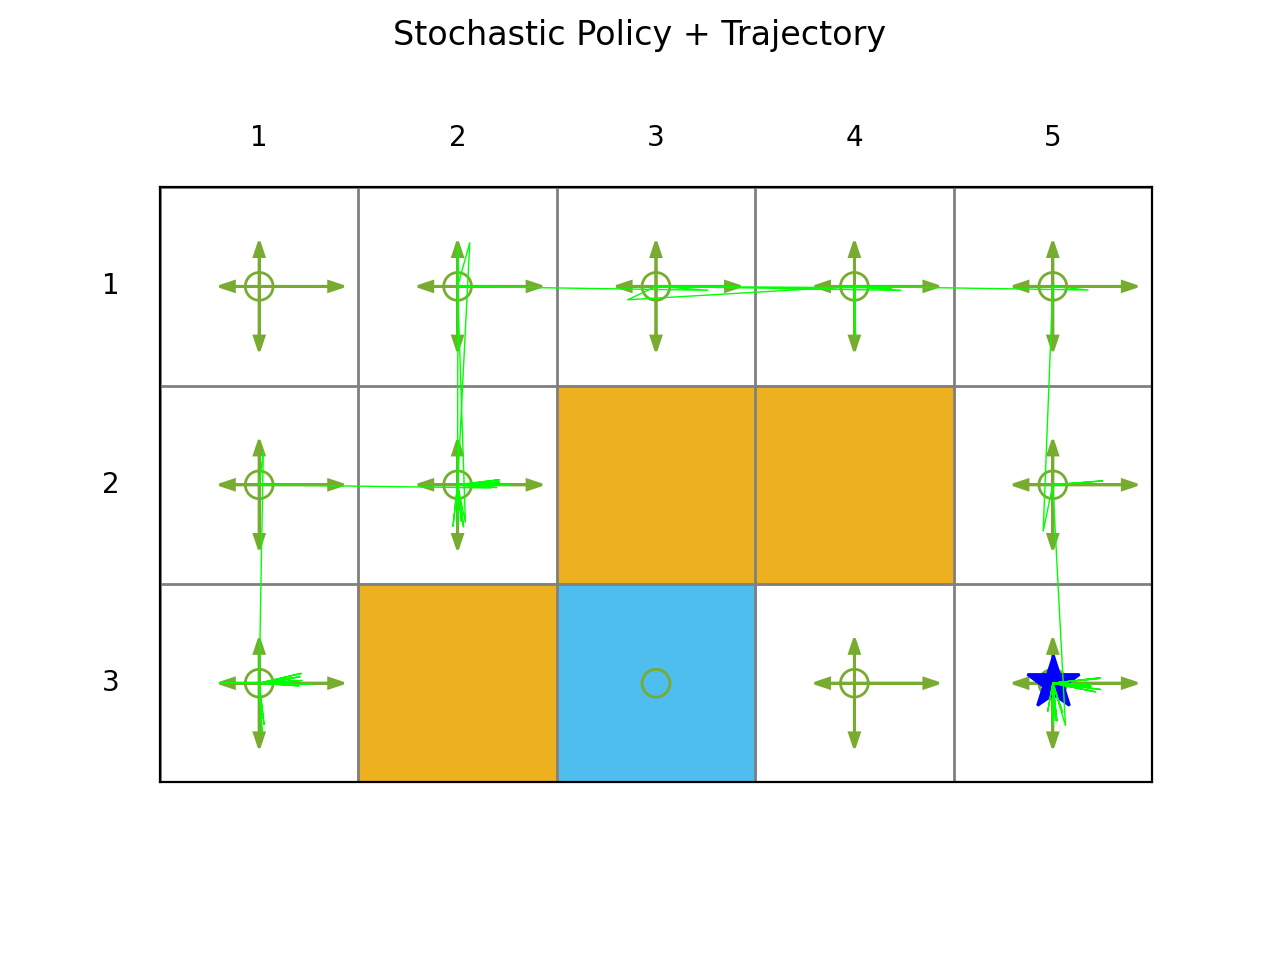
\includegraphics[width=0.7\textwidth]{stochastic_policy_trajectory.png}
\caption{Visualization of the stochastic policy and the resulting trajectory from start state (0, 2).}
\label{fig:stochastic}
\end{figure}

The first 10 states of the trajectory are:
\begin{verbatim}
[(0, 2), (0, 2), (0, 2), (0, 2), (0, 2),
 (0, 2), (0, 2), (0, 2), (0, 2), (0, 2)]
\end{verbatim}

\subsection{Discounted Return}
The calculated discounted return for this 50-step trajectory is:
$$ G = -8.771119968050847 $$

\section{Observations and Discussion}

The results from the two policies show a stark contrast in performance, highlighting the difference between an informed, optimal policy and a naive, random one.

\begin{itemize}
    \item \textbf{The Deterministic Policy} performed exceptionally well. It successfully navigated the agent from the start state (0, 2) to the target state (2, 2) by following the shortest possible path while avoiding all forbidden zones. The positive discounted return of \textbf{3.82} reflects this success; the agent reached the target and accumulated high rewards, discounted over time. This demonstrates the power of having a model of the environment (the grid layout) to compute an optimal plan.

    \item \textbf{The Stochastic Policy} performed very poorly. The trajectory shows the agent never left the starting state (0, 2). This is because from state (0, 2), the actions with the highest probabilities are "right" (0.5) and "down" (0.3). The "right" action leads to state (1, 2), which is a forbidden zone, and the "down" action leads off the grid. In both cases, the environment rules dictate that the agent does not move and receives a reward of -1. Therefore, the agent had a high probability (0.5 + 0.3 = 0.8) of receiving a penalty and remaining in the same state at each step. This created a "trap," leading to a highly negative discounted return of \textbf{-8.77} as it accumulated penalties over 50 steps.
\end{itemize}

In conclusion, a policy that intelligently uses the structure of the environment (like the BFS-based deterministic policy) is far superior to a policy that acts randomly without regard to consequences. The stochastic policy's failure highlights how an agent with a poor policy can \textbf{become trapped} in parts of the state space that yield low or negative rewards.





\newpage

\section{Key Code Implementation}

\subsection{Discounted Return Calculation}
This function calculates the discounted return G based on the list of rewards collected during an episode and a given discount factor gamma, following the formula $G_t = \sum_{k=0}^{T-1} \gamma^k R_{t+k+1}$.

\begin{lstlisting}[language=Python, caption={Code for calculating the discounted return.}]
def calculate_discounted_return(rewards, gamma):
    """
    Calculates the discounted return for a list of rewards.

    Args:
        rewards (list): A list of rewards from the trajectory.
        gamma (float): The discount factor.

    Returns:
        float: The calculated discounted return G.
    """
    G = 0.0
    for t, r in enumerate(rewards):
        G += (gamma ** t) * r
    return G
\end{lstlisting}

The core logic for generating the two policies is encapsulated in the following functions.

\subsection{Deterministic Policy Generation}
This function uses BFS to find the shortest path from all states to the target, then builds a policy matrix that follows this path.

\begin{lstlisting}[language=Python, caption={Code for building the deterministic policy.}]
def build_deterministic_policy(env):
    """
    Deterministic policy using a maze-solving method:
    - Use BFS to find the shortest path from each reachable state to the target_state.
    - The policy selects the first action along this shortest path.
    - For forbidden or target states, the policy is to 'stay'.
    Returns a matrix of shape = (num_states, num_actions).
    """
    num_states = env.num_states
    num_actions = len(env.action_space)
    policy = np.zeros((num_states, num_actions))

    stay_idx = env.action_space.index((0,0))

    # Pre-calculate the parent of each state on the shortest path using BFS
    target = tuple(env.target_state)
    queue = deque([target])
    parent = {target: None}

    while queue:
        current = queue.popleft()
        for action in env.action_space:
            if action == (0,0):  # skip stay
                continue
            prev = (current[0] - action[0], current[1] - action[1])
            if (0 <= prev[0] < env.env_size[0] and
                0 <= prev[1] < env.env_size[1] and
                prev not in env.forbidden_states and
                prev not in parent):
                parent[prev] = current
                queue.append(prev)

    # Build the policy
    for s in range(num_states):
        st = env.idx_to_state[s]

        if st in env.forbidden_states or st == target or st not in parent:
            policy[s, stay_idx] = 1.0
            continue

        # Find the next step on the path
        next_state = parent[st]
        dx = next_state[0] - st[0]
        dy = next_state[1] - st[1]
        action = (dx, dy)
        if action in env.action_space:
            a_idx = env.action_space.index(action)
            policy[s, a_idx] = 1.0
        else:
            policy[s, stay_idx] = 1.0

    return policy
\end{lstlisting}

\subsection{Stochastic Policy Generation}
This function assigns a fixed probability distribution to every non-terminal state. It's a simple, non-learning policy.

\begin{lstlisting}[language=Python, caption={Code for building the stochastic policy.}]
def build_stochastic_policy(env):
    """
    Example of a stochastic policy (with a bias for right and down):
    - For non-terminal, non-forbidden states: Right 0.5, Down 0.3, Up 0.1, Left 0.05, Stay 0.05
    - For forbidden or target states: the probability of 'stay' is 1
    Returns a matrix of shape (num_states, num_actions)
    """
    num_states = env.num_states
    num_actions = len(env.action_space)
    policy = np.zeros((num_states, num_actions))

    weight_map = {}
    weight_map[(1,0)] = 0.5   # right
    weight_map[(0,1)] = 0.3   # down
    weight_map[(0,-1)] = 0.1  # up
    weight_map[(-1,0)] = 0.05 # left
    weight_map[(0,0)] = 0.05  # stay

    for s in range(num_states):
        st = env.idx_to_state[s]
        if st == tuple(env.target_state) or st in env.forbidden_states:
            stay_idx = env.action_space.index((0,0))
            policy[s, stay_idx] = 1.0
        else:
            # Create probability distribution based on weight_map
            probs = np.array([weight_map.get(a, 0.0) for a in env.action_space])
            probs = probs / probs.sum()
            policy[s, :] = probs
    return policy
\end{lstlisting}

\end{document}